\documentclass[conference,final,a4paper,twocolumn,9pt]{IEEEtran}

\usepackage{cmap}
\usepackage[utf8x]{inputenc}
\usepackage[T1]{fontenc}

\usepackage{lmodern}

\usepackage{mathtools}
\usepackage{amssymb}

\usepackage[USenglish]{babel}

\usepackage{array}
\usepackage{amsthm}
\usepackage{amsfonts}
\usepackage{mathtools}
\usepackage{makeidx}
\usepackage[pdftex]{graphicx}
\usepackage{url}
\usepackage{epigraph}
\usepackage{hyperref}
\usepackage{natbib}

\ifCLASSINFOpdf
\usepackage[pdftex]{graphicx}
\DeclareGraphicsExtensions{.pdf,.jpeg,.png}
\else
\usepackage[dvips]{graphicx}
\DeclareGraphicsExtensions{.eps}
\fi

\usepackage{amsmath}
\usepackage{algorithmic}
\usepackage{url}

\usepackage{tikz, pgfplots}
\usepackage{tikz-qtree}

\usetikzlibrary{patterns}

\begin{document}
\title{RobOptim: an Optimization Framework for Robotics}

\author{\IEEEauthorblockN{Thomas Moulard}
\IEEEauthorblockA{FIXME}
\and
\IEEEauthorblockN{Florent Lamiraux}
\IEEEauthorblockA{FIXME}
\and
\IEEEauthorblockN{Karim Bouyarmane}
\IEEEauthorblockA{FIXME}
\and
\IEEEauthorblockN{Eiichi Yoshida}
\IEEEauthorblockA{FIXME}}

\maketitle

\begin{abstract}
\boldmath
The abstract goes here.
\end{abstract}

\IEEEpeerreviewmaketitle

\section{Introduction}\label{sec:introduction}


Over the past years, numerical optimization proved itself particulaly
suited for various robotics use such as posture or trajectory
optimization, robot control and more. These applications yield both
linear and non-linear optimizations problems with equalities and
inequalities constraints. Robot control also relies on other types of
optimization problems such as quadrating programming. As these
algorithms must run in real-time, it leads to strong constraints on
the implementation efficiency. The design and implementation of a
solver is tedious and error-prone. Avoiding numerical precision
issues, assuring that the algorithm behaves properly in all cases and
reports correctly the errors it may encounter is challenging, in
particular for roboticians which are not experts in optimization
techniques. Among available optimization toolboxes, the Matlab
Optimization Toolbox[CITE], the Open Optimization library, OPT++,
IPOPT, SciPy and the GSL (Gnu Scientific Library) all provides some
optimization algorithms. Unfortunately, these libraries suffer from
several drawbacks: difficult to use, no support for advanced
algorithms such as support for constrained optimization, efficiency
issues, etc. They also all lack a unified model expressing
optimization problems.


RobOptim solves these limitations by introducing a model allowing to
express any continuous optimization problem, constrained or not. Its
design was focused on providing an easy to use C++ set of libraries, a
safe and efficient framework which can be used to prototype robotics
applications. The RobOptim computational model will be first
introduced in~\autoref{sec:roboptim} and different applications will
be detailed in~\autoref{sec:application}. In particular, an extension
of RobOptim for a particular type of problem has been realized
recently, demonstrating the ability of RobOptim to support a variety
of problems. The conclusion will detail feedback from current users of
RobOptim and present the roadmap for the next developments.


\section{RobOptim overview}\label{sec:roboptim}


RobOptim is a set of open-source C++ libraries licensed under the LGPL
license. Code source, documentation and examples are available on the
project webpage: \mbox{\url{http://www.roboptim.net/}}.


The RobOptim framework is divided into three parts. The core layer
provides a computation model expressive enough to model different
types of optimization problems. The solver layer gathers different
optimization algorithms which are.


\subsection{Mathematical functions representation}


Continuous optimization problems can be defined as follow:

\begin{equation}\label{eq:optimization}
  \min_{\mathbf{x} \in \mathbb{R}^n} f(\mathbf{x}) \text{ under the constraint } \mathbf{x} \in \mathbf{X}
\end{equation}

where $f : \mathbb{R}^n \mapsto \mathbb{R}$ is the cost function and
$\mathbf{X} \subset \mathbb{R}^n$ is the space of the admissible
solutions. This space is usually defined by a set of inequality and
equality constraints:

\begin{equation}
  \mathbf{X} \equiv \left\{
  \begin{array}{l l}
    c_i (x) = 0    & \quad i \in \xi \\
    c_j (x) \leq 0 & \quad j \in \nu \\
  \end{array} \right.
\end{equation}

$c_i$, $c_j$ are respectively the set of equality and inequality
constraints. $i$ and $j$ are the indices identifying the constraints.

The mathematical functions $f$ and $c_k$, $k \in \xi \cup \nu$ must
provide a way to evaluate their result at any point they are
defined. Their associated gradient and hessian may also be
provided. To finish, each of these function may have a particular
structure that can help the resolution. The goal of the RobOptim core
layer is to express these features through the C++ typing rules.


Depending on the solving algorithm, it may be necessary to obtain the
jacobian and in some cases even the hessian of the used
functions. Hence, a function which provides the maximum information
about itself will be usable with a larger proportion of solvers.

\begin{figure}
  \begin{center}
    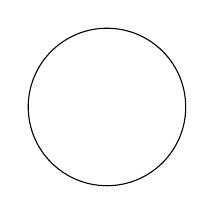
\begin{tikzpicture}
      \draw (0,0) circle (1) ;
    \end{tikzpicture}
  \end{center}
  \caption{Sets representing the different kind of functions that
    RobOptim can model out-of-the-box.}\label{fig:functions}
\end{figure}

In RobOptim, each mathematical function is represented by a different
C++ class. All of these types then inherit from the abstract kind of
mathematical functions they represent. The following kind of
mathematical functions are bundled with RobOptim core: function that
can evaluate itself (Function type), function evaluate itself and its
gradient (DifferentiableFunction), function that can evaluate itself,
its gradient and its hessian (TwiceDifferentiableFunction), etc.  Let
'A <: B' denote the relationship ``type B is a subtype (subclass) of
A'' or ``B inherits from A''. Then a partial order can be defined
where: Function <: DifferentiableFunction <:
TwiceDifferentiableFunction. It can also be understood through sets
as illustrated by~\autoref{fig:functions}.


\subsection{Optimization problem definition and problem resolution}


Once function cost and all constraints functions have been
implemented, an optimization problem has to be built. RobOptim core
provides a meta-class Problem parametrized by two parameters $F$ and
$C_L$. $F$ is the type of the cost function and $C_L$ is the list of
the constraints types. A non-linear problem with constraints then has
the following type:


\texttt{Problem<DerivableFunction, vector<LinearFunction, DerivableFunction > >}


The constraints can be either linear or non-linear. With this
constraint type definition, the constraints will be divided into two
categories which will help the solver to perform efficiently.

Additionally, bounds can be set on the optimization variables and a
starting point for the optimization process can be set. When the
constraints are added to the problem, each constraint is associated
with an interval. If this interval is reduced to a point, the
constraint is an equality constraint. At each time of the problem
construction at both compile time and run-time, RobOptim checks that
only valid problem are built. For instance if one add a constraint of
type $T$ then RobOptim checks at compile time that the constraint is a
subtype of $T$.


Once the problem is defined, a solver need to be instantiated that
will solve the problem. Each solver is parametrized by the same
variables than an optimization problem. Therefore the solver
$S<P_1,C_{L1}>$ can solve the problem $P<P_2,C_{L2}>$ if the following
relation is true:


\begin{equation}
  P_1 <: P_2 \wedge \forall i, C_{L1}(i) <: C_{L2}(i)
\end{equation}


Basically, the problem can be solved if all types provide enough or
more information than necessary. For instance if gradient are
required, the function may also provide hessian computation but if
gradient are lacking the compile time assertions will fail and prevent
the user from building an invalid optimization problem.

By separating problem expression from solver, dynamic changes of the
solving algorithm are possible. Each solver is bundled as a plug-in
which is loaded at run-time. An interest is to let the user change its
problem complexity during its design process freely. Other frameworks
would require a different API depending on the kind of optimization at
hand, here the changes are minimal. One may choose to use a more
powerful than required solver at first and then refince their choice
or implement later a new plug-in providing the best algorithm for one
particular application. These features are provided through
meta-programming techniques and come with a near zero
cost\footnote{RobOptim core do not realize copy so the additional
  runtime cost is only due to calls to virtual functions.} at runtime
and are unique to RobOptim.

\subsection{Costs and constraints toolbox}


Unlike others frameworks where computations are tightly linked to one
problem and one solver, the abstraction layer of RobOptim allows user
to implement toolboxes of reusable functions. This part of RobOptim is
dedicated to robotics. The ``trajectory'' layer of RobOptim is
currently providing trajectores defined as B-Splines and associated
mathematical functions to realize minimal time optimization for
instance.


\subsection{Toward easy and safe problem design}


FIXME

\section{Applications and case study}\label{sec:application}


RobOptim has been used to solve several different types of numerical
optimization problems applied to robotics. The two scenarii that will
be detailed here are footsteps optimization and posture optimization
for a humanoid robot. Another important point is the extensibility of
the framework. To demonstrate RobOptim capacities to adapt to new
types of optimization problems an example of such extension will be
given.
\subsection{Step planning for humanoid robots}


Generating a walking motion in an environment cluttered with obstacles
is challenging. One commonly used approach are random searching
trees. These probabilistic algorithm will try to create a path between
the starting point and the goal point by sampling configurations
randomly. This family of algorithms have the ability to find solutions
for highly dimensioned problems on a reasonable time. However, the
random nature of these algorithms tend to produce paths which are not
``human-like''. One solution to improve these paths is numerical
optimization. Instead of considering the whole body trajectory,
RobOptim has been used to optimize a biped robot walking trajectory
determined beforehand by a motion planning algorithm.

Let $\gamma$ be the initial robot waist trajectory defined as a
B-Spline from $t_{min}$ to $t_{max}$. A free time trajectory $\Gamma$
is defined from $T_{min}$ to \linebreak $T_{max} = T_{min} + \lambda
(t_{max} - t_{min})$ as
\begin{equation}
  \Gamma_{\lambda} (T) = \gamma (t_{min} + \frac{1}{\lambda} (T -
  T_{min}))
\end{equation}

\begin{figure}
  \begin{center}
    \begin{tabular}{|c|l l l| l |l l l|}
      \hline
      Time
      & \multicolumn{3}{|c|}{control point 1}
      & \ldots
      & \multicolumn{3}{|c|}{control point $n$}\\
      \hline
      $\lambda$
      & $x_0$ & $y_0$ & $\theta_0$
      & \ldots
      & $x_n$ & $y_n$ & $\theta_n$\\
      \hline
    \end{tabular}
  \end{center}
  \caption{Optimization variables for walking motion problem\label{fig:optim-param}}
\end{figure}


The use of a free time trajectory allows the solver to both optimize
trajectory shape and speed by respectively changing the control points
and the scale $\lambda$. Optimization variables are illustrated
by~\autoref{fig:optim-param}. The free time trajectory derived from
the initial trajectory $\gamma$ is used as the state of the solver.


\begin{figure}
  \begin{center}
    \begin{tabular}{|c|c|}
      \hline Cost function & $f(\mathbf{x}) = \lambda$\\ Speed
      constraint & $\forall T, \text{foot},\quad
      (\frac{v_{\text{foot}}^{x}}{v_{\text{max}}^{x}})^2 +
      (\frac{v_{\text{foot}}^{y}}{v_{\text{max}}^{y}})^2 - 1 \leq
      0$\\ Distance constraint & $\forall T,\quad\text{distance} (\text{obstacle},
      \Gamma (T)) > 0$\\ \hline
    \end{tabular}
    \caption{Walking optimization problem formulation\label{fig:pb-walking}}
  \end{center}
\end{figure}


The problem cost function is defined as $\lambda$. It corresponds to
minimizing the time by accelerating the trajectory as much as
possible. To ensure that the final trajectory stay feasible while
encouraging forward motion, a speed constraint is added which take
separately into account the front speed $v^x$ and the lateral speed
$v^y$ of each foot of the robot. Another constraint is preventing the
robot to collide with environment obstacles. The problem definition is
detailed in~\autoref{fig:pb-walking}.


\begin{figure}
  \begin{center}
    %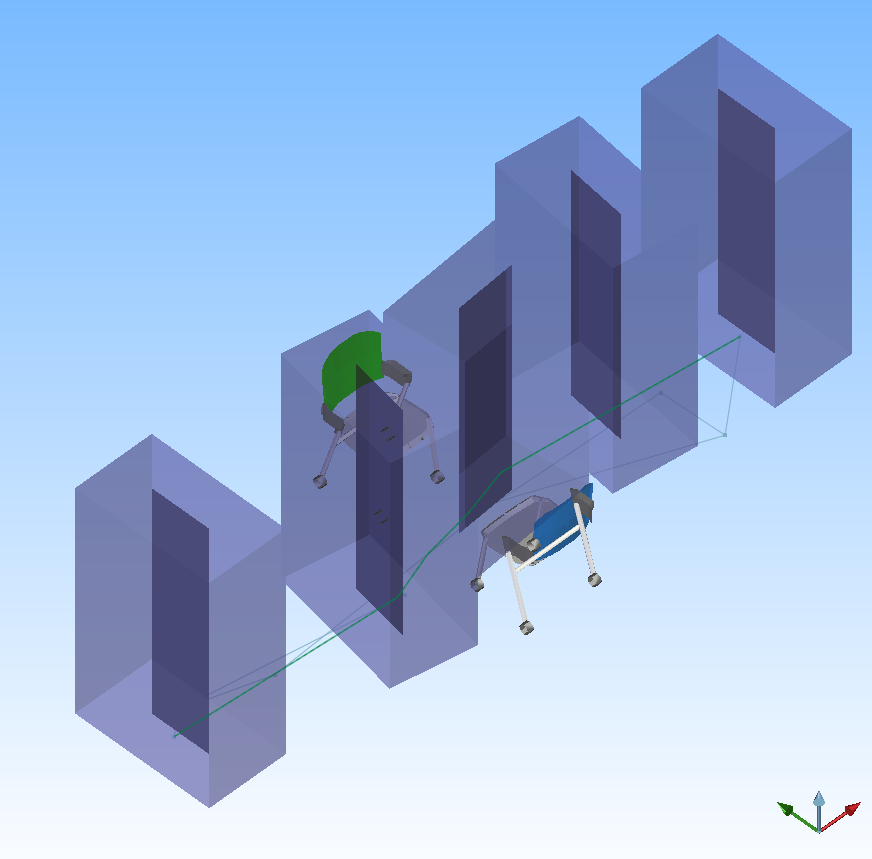
\includegraphics[width=\linewidth]{two-chairs.png}
    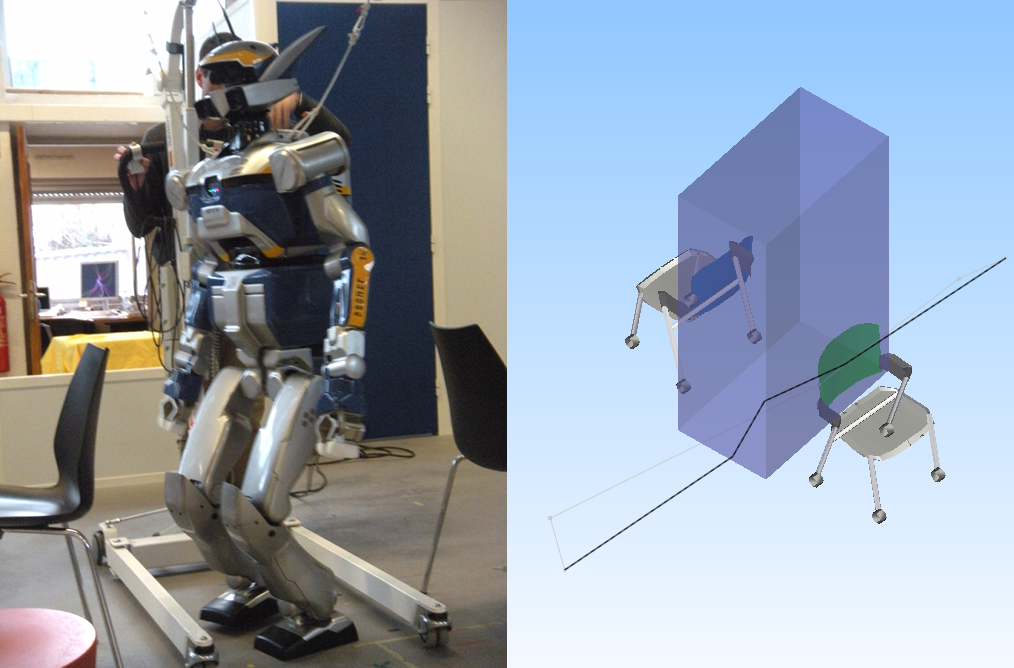
\includegraphics[width=\linewidth]{hrp2-two-chairs.png}
    \caption{Walking trajectory optimization\label{fig:result-walking}}
  \end{center}
\end{figure}


This non-linear problem has been successfully solved by RobOptim while
relying on the proprietary solver CFSQP and result is show
on~\autoref{fig:result-walking}.


\subsection{Posture optimization for humanoid robots}


\begin{figure}
  \begin{center}
    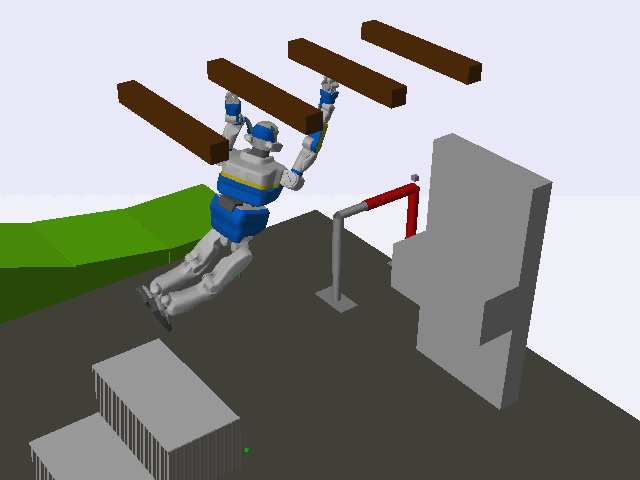
\includegraphics[width=\linewidth]{agent-067.jpg}
    \caption{Posture optimization\label{fig:stence-optimization}}
  \end{center}
\end{figure}


Another problem is posture optimization, which consists in choosing
the best configuration such that a system will accomplish the
objectives it has been assigned. In this example, the goal is to find
a configuration as close as possible to a goal posture while taking
into account various constraints. In this case, robots and objects
environment are considered as elements of the optimization
problem. Constraints include: robot and objects static equilibrium,
Newton's third law, Coulomb friction model, fixed grasp model for
bilateral contact forces, joints limits and torques limits. This
problem is described extensively
in~\cite{DBLP:conf/icra/BouyarmaneK11} and demonstrated the ability of
RobOptim to solve complex large scale non-linear problems.


\subsection{Extending the framework: least square optimization}


Initially, non-linear optimization problems with constraints have been
solved with RobOptim. By providing a generic computational framework,
the initial infrastructure has been extended to other types of
optimization problems such as least square problems. In least square
problems, cost function can be expressed as:

\begin{equation}
  f(\mathbf{x}) = \sum_i (\mathbf{x}_i - \mathbf{x}^{ref}_i)^2
\end{equation}


Another function type called \texttt{SumOfC1Squares} has been derived
from the \texttt{DifferentiableFunction} class. The CMinPack solver
has then been wrapped into a RobOptim solver class which takes as
input problem of the type: \texttt{Problem<SumOfC1Squares, vector<> >}
which means that the cost function must be a sum of squares while
constraints are not supported for this particular type of problems.

The introduction of this new set of feature did not require any change
in the RobOptim structure and proved the genericity of our approach.


\section{Conclusion}\label{sec:conclusion}


A new approach to optimization problem representation has been exposed
in this paper. By expressing numerical optimization problems through
C++ typing, the RobOptim optimization framework provides a unified
computational model. Moreover, through advanced C++ template
meta-programming, efficiency is preserved while giving the capacity to
express high-level mathematical objects such as cost functions and
constraints. These features have been proved useful to solve different
types of robotics problem. Even while being generic, the RobOptim core
layer suffers from limitions. It still lacks support for optimization
in non-scalar spaces such as $\text{SO}(3)$. By importing knowledge
about the structure of the optimization variables, solvers could
realize more efficient computation. For instance, 3d rotations can be
represented by homogeneous matrices, quaternions, vector and angle,
etc. Switching from one representation to another may lead to better
convergence and a decrease in the number of necessary mathematical
operation. One goal would be to both be able to express information
regarding the optimization variables structure and find a method to
help solvers rely on these additional information. To achieve this
level of expressiveness, taking part of modern C++ feature is
mandatory and no optimization framework is providing yet this kind of
help when designing an optimization problem.


To conclude, RobOptim is a step forward toward making optimization
techniques available for non-expert users by providing an easy to
understand and generic model, strong C++ typing ensuring safety and
toolboxes containing robotics oriented functions that may be reuse
when building its own optimization problem.


\section{Bibliography}\label{sec:bibliography}
\bibliography{robomec13.bib}

\end{document}
